\documentclass[a4paper,10pt,fleqn]{article}
\usepackage{mathtext}
\usepackage[T2A]{fontenc}
\usepackage[utf8x]{inputenc}
\usepackage[english,ukrainian]{babel}
\usepackage{amsfonts,amsmath,stmaryrd}
\usepackage{indentfirst}
\usepackage[pdftex]{color,graphicx}
\usepackage{float}
\usepackage{subfig}
\usepackage[protrusion=true,expansion=true]{microtype}

\DeclareGraphicsRule{.jpeg}{.bmp}{}{}
\textwidth 16 cm
\textheight 24.5cm
\topmargin -1 cm
\evensidemargin 0 cm
\oddsidemargin 0 cm

\title{Індуктивні методи моделювання навігації агента}
\author{Накрийко Андрій}

\begin{document}
\selectlanguage{ukrainian}
\maketitle

\section{Вступ}

Потреба керування автономними механізмами виникає постійно в різноманітних областях діяльності людини. Це можуть бути як надскладні та небезпечні завдання, такі як: космічні експедиції, дослідження підземних озер, жерл вулкану тощо, так і менш небезпечні, які, тим не менше, так само необхідні та важливі, наприклад: домашні та промислові роботи, інтелектуальні системи тощо. Ці задачі є предметом досліджень різноманітних галузей науки: теорії керування, теорії прийняття рішень, робототехніки, штучного інтелекту, машинного навчання тощо. За останні 20 років людство зробило суттєві кроки вперед у вирішенні цих задач, проте повністю вирішеною проблему вважати ще зарано.

У цій статті ми розглянемо одну з задач, яку потрібно розв'язувати в багатьох застосуваннях, а саме "--- проблему навігації агента в середовищі, попередніх даних про яке немає. Буде описано два підходи до її розв'язання та результати їх застосування у практичних експериментах.

\section{Постановка задачі}

Для більшої конкретності, агентом у нашому випадку був обраний автомобіль, тому нашою задачею є реалізація системи контролю автомобіля, яка забезпечує безперервний рух у віртуальному середовищі з огинанням перешкод. Щоб якомога краще наблизити умови, в яких перебуває віртуальний автомобіль, до реальності, система керування сприймає лише об'єкти, які потрапляють у поле зору, обмежене певним кутом та дальністю огляду. Агенту надається інформація про те, наскільки близько знаходиться перешкода в межах кожного з трьох секторів ``поля зору'' (\ref{fig:visible-area}). Ці значення знаходяться в межах від $0$ до $1$, при цьому одиниця означає, що перешкоди немає або ж вона знаходиться на самій границі поля зору. Керування полягає у виборі в кожен момент часу значення прискорення з діапазону $[-1,1]$ ($-1$ "--- максимальне гальмування, $1$ "--- максимальне допустиме прискорення вперед) та кута повороту керма, також з діапазону $[-1,1]$. Таким чином, вхідними даними є багатовимірний вектор про дальність перешкод в межах поля зору, а вихідними даними "--- двовимірний вектор прискорення та кута повороту. Усі координати векторів неперервні. 
\begin{figure}
  \centering
  \subfloat[Поле зору автомобіля]{
  	\label{fig:visible-area}
  	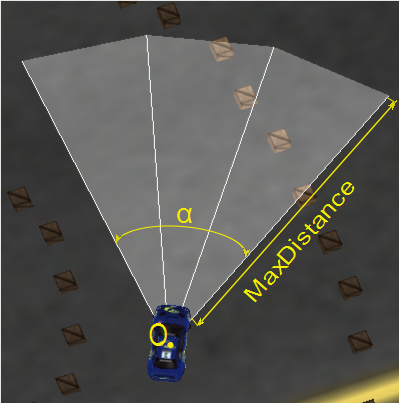
\includegraphics[width=0.38\textwidth]{visible-area}
  }\,
  \subfloat[Автомобіль застряг]{
  	\label{fig:car-stuck}
  	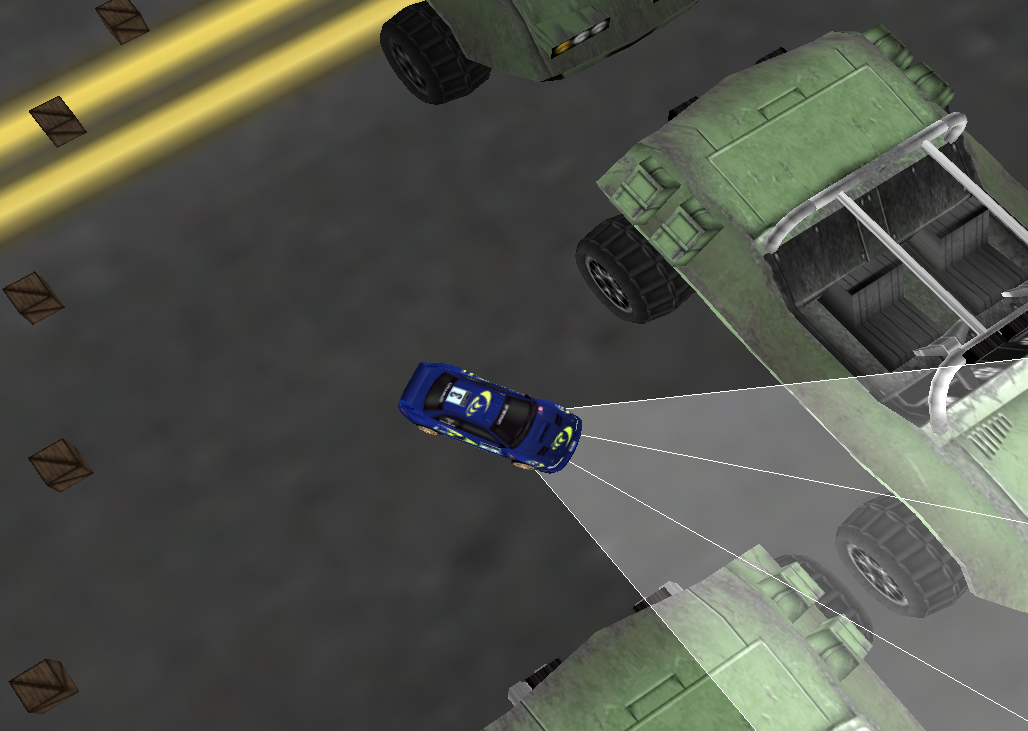
\includegraphics[width=0.54\textwidth]{car-stuck}
  }
  \caption{Ілюстрації до першого підходу}
  \label{fig:car-related}
\end{figure}

\section{Експертні правила та штучна нейронна мережа}

Першим підходом до розв'язання задачі керування агентом було використання наперед заданого набору експертних правил, що представляли собою пари еталонних вхідних (представлення певної ситуації) та відповідних вихідних даних (оптимальне керування). Для узагальнення скінченного набору правил на усю множину можливих ситуацій була використана нейромережа, яка виконувала роль апроксиматора функції керування. Завдяки узагальнюючій властивості нейромережі, можна надіятися отримати контролер, який здатний приймати ``осмислені'' рішення в ситуаціях, для яких не було надано експертних правил, якщо в еталонному наборі є правила, які описують ситуації, близькі до даної.

Для перевірки ефективності рішення на основі експертних правил, було створено віртуальне середовище, в якому рухався автомобіль, з достатньо реалістичної фізикою. Завданням агента було забезпечення безперервного руху в межах середовища без натикання на нерухомі перешкоди. При цьому час вважався неперервним, тобто рішення про подальші дії приймалися не через однакові дискретні проміжки часу, а як тільки було можливим. Така особливість вносить певну залежність поведінки агента від потужності комп'ютера, на якому виконується симуляція, оскільки більш потужний комп'ютер дає можливість більш точного керування внаслідок частішого прийняття рішень про подальший рух агента. 

Як буде зазначено пізніше, при використанні самонавчання постановка задачі була дещо зміненою внаслідок особливості парадигми навчання з підсиленням, а також час вважався дискретним. 

\subsection{Результати підходу на основі експертних знань}

Результати не можна охарактеризувати однозначно. З однієї сторони, система контролю на базі нейромережі досить адекватно керувала автомобілем з доволі складною фізикою, успішно оминаючи перешкоди та забезпечуючи безперервний рух автомобіля в середовищі, про яке вона не мала жодної попередньої інформації. Більше того, для підвищення рівня ``природності'' керування, системі контролю надавалася лише інформація про об'єкти, які попадали в поле зору автомобіля, що являло собою сектор з визначеним радіусом (дальністю бачення) та центральним кутом (кутом огляду). Базуючись лише на даних про віддаль до найближчих об'єктів в полі зору, система контролю забезпечувала завчасне оминання перешкоди з плавною зміною швидкості та напрямку руху автомобіля. Очевидно, що велику роль в досягненні вказаної природності та адекватності керування відіграла вдало підібрана множина еталонних правил, що становила собою навчальну множину для нейромережі.

З іншого боку, найбільшою проблемою, з якою довелося зіткнутися, була наявність ситуацій, в яких автомобіль зупинявся і система контролю не могла вивести його з нерухомого стану. Одна з таких ситуацій подана на рис.~\ref{fig:car-stuck}, в якій автомобіль заїхав у глухий кут і застряг, не зумівши здійснити розворот назад. Цю проблему, теоретично, можна було б розв'язати, ввівши у стан системи значення поточної швидкості та задавши додаткові експертні правила, які б враховували такі ситуації і дозволяли автомобілю здійснити розвертання у разі застрягання. Проте на практиці це достатньо проблематично, оскільки введення додаткової змінної стану призводить до ускладнення поведінки всієї системи, підвищення рівня вимог до точності та репрезентативності експертних правил. Більше того, для того, щоб зробити розвертання автомобіля безпечнішим та природнішим, довелося б вводити також змінні, які б відповідали за задній огляд автомобіля, що призводить до ще більш строгих вимог до експертних правил.

Слід зазначити, що ще однією причиною (окрім вказаної обмеженості визначеного стану динамічної системи) такої поведінки є особливість фізичної моделі автомобіля. Мається на увазі природа автомобіля "--- для того щоб здійснити поворот, чи тим більше розворот, автомобіль повинен рухатись вперед або, відповідно, назад, що в умовах, коли вже відбулося застрягання, дуже проблематично. Можливим розв'язанням даної проблеми є зміна типу транспортного засобу. Якщо взяти транспортний засіб, здатний здійснювати поворот (а отже і розворот) на місці, то можна значно зменшити ймовірність його застрягання. Таким транспортним засобом, для прикладу, може бути танк, в якому шляхом незалежного обертання гусениць в різні сторони можна домогтися розвороту на будь-який кут, залишаючись при цьому на місці.

Важливою проблемою, що постає при вказаному підході, є вибір внутрішньої структури нейромережі. Якщо використати недостатню кількість нейронів, то нейромережа не зможе в достатній мірі вивчити набір правил і, відповідно, не зможе повністю використати експертні знання. З іншого боку, використовуючи надто велику кількість нейронів, існує загроза надто точного запам'ятовування (overfіttіng) правил без належного узагальнення їх на схожі ситуації. В такому випадку нейромережа буде точно виконувати правила в описаних ситуаціях, але навіть незначна зміна ситуації призведе до неадекватної зміни керування.

Таким чином, при використанні експертних правил, з'являється велика кількість практичних питань, на які немає чітких теоретичних відповідей, а все доводиться вирішувати в результаті численних експериментів. Саме тому було вирішено випробувати інший підхід, який би не вимагав трудомісткого та складного процесу вибору репрезентативних експертних правил "--- самонавчання на основі досвіду безпосередньої взаємодії з середовищем.

\section{Самоорганізаційний підхід "--- навчання з підсиленням}

Оскільки використання попереднього підходу сильно залежить від якості навчальної вибірки (експертних правил), що при найменшому ускладненні сприйняття агентом середовища призводить до значних ускладнень експертних правил, було вирішено відійти від моделі навчання з учителем. Натомість був використаний самоорганізаційний підхід. Основна ідея такого підходу полягає в тому, щоб дати можливість агенту розробити власну ''внутрішню систему правил'' щодо оптимальної поведінки в середовищі в результаті безпосередньої взаємодії з ним. Взаємодіючи з середовищем, агент отримує певний досвід і, якщо задати певний механізм оцінки агентом власних дій, то в результаті достатньої кількості ``досвіду'', можна надіятися, що агент розробить ефективну стратегію поведінки. Такий підхід отримав назву \emph{навчання з підсиленням (reіnforcement learnіng)}. При використанні навчання з підсиленням відпадає необхідність в розробці системи експертних правил, хоча, натомість, виникає проблема вибору ефективної та точної системи оцінки дій агента. Проте, для достатньо складних систем, зазвичай, значно легше визначити механізм оцінки дій, аніж розробити повну та якісну систему правил.

Навчання, в процесі якого агент розробляє систему правил в результаті багаторазової взаємодії з середовищем, є індуктивним, оскільки корисна інформації ''видобувається'' з необробленої інформації про середовище (інформація про віддалі до перешкод, сигналізація зіткнень тощо). Дедуктивний ж процес навчання, використаний у попередньому підході, для розроблення внутрішньої системи правил використовував структуровану та оброблену інформацію про середовище, подану у вигляді готових еталонних правил. Слід зазначити, проте, що в даному випадку дедуктивний процес частково включав і індуктивний підхід, оскільки нейромережа свою внутрішню структуру вибудовувала також з необроблених (з точки зору нейромережі) даних. Проте в загальному, експертний підхід - дедуктивний за своєю суттю. 

Далі ми детальніше зупинимося на індуктивному підході та на результатах його практичного застосування.

\subsection{Загальні поняття навчання з підсиленням}

Ідея навчання з підсиленням полягає в наступному. Існує дві сутності "--- середовище та агент, що діє у ньому. Агент певним чином здатний сприймати середовище та має набір можливих дій, якими він здатний змінювати середовище. Уся сукупність інформації, доступна агенту в кожен дискретний момент часу $t$, називається \emph{станом} і позначається $s_t$. Відповідно можна ввести поняття множини усіх можливих станів середовища $\mathcal{S}\ (s_t \in \mathcal{S})$. Слід зазначити, що множина можливих станів може бути як дискретною, так і неперервною, а отже і нескінченною. При цьому в більшості реальних застосувань множина станів нескінченна. Також визначимо множину \emph{дій} агента, які допустимі в стані $s_t$ "--- $\mathcal{A}(s_t)$. Множина допустимих дій також в загальному випадку може бути нескінченною.

\begin{figure}
\centering
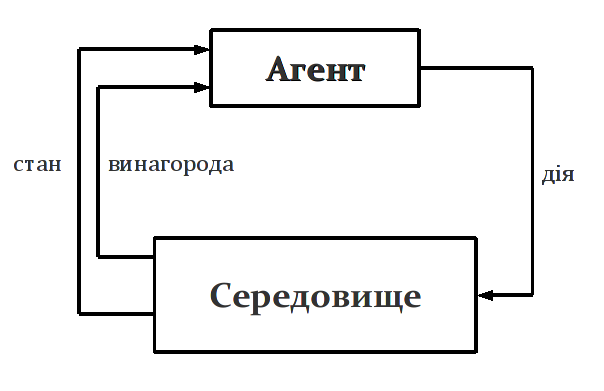
\includegraphics[width=0.5\textwidth]{agent-env-diagram.png}
\caption{Схема взаємодії агента та середовища}
\label{fig:agent-env-diagram}
\end{figure}
Схематично взаємодію агента та середовища представлено на рис.~\ref{fig:agent-env-diagram}. В дискретний момент часу $t$ агент отримує стан середовища $s_t \in \mathcal{S}$, на основі цієї інформації він вибирає і здійснює певну дію $a_t \in \mathcal{A}(s_t)$, в результаті чого отримує певне значення миттєвої винагороди $r_t \in \mathbb{R}$ від середовища. Метою агента в такій системі є визначення для кожної можливої ситуації $s_t$ такої дії $a_t$, яка приводить до максимізації сумарної винагороди в довготерміновому періоді (\emph{очікуваного прибутку} $R_t$). Більш формально це можна визначити так. Потрібно визначити відображення $\pi:\mathcal{S}\times\mathcal{A} \rightarrow [0,1]$, яке називається \emph{стратегією}, таке, що $\pi(s, a)$ визначає ймовірність здійснення дії $a$ при перебуванні агента у стані $s$. В випадку детермінованої стратегії, $\pi(s,a) \in \{0,1\}$. Стратегія $\pi$ називається \emph{оптимальною}, якщо для будь-якого стану послідовність дій, визначена нею, призводить до максимального очікуваного прибутку.

Визначимо більш точно поняття прибутку. Нехай, починаючи з часу $t$, агент отримує послідовність винагород $r_{t}, r_{t+1}, r_{t+2}, \ldots$. Тоді основною метою агента буде максимізація \emph{прибутку} $R_t$, де $R_t$ "--- це певна функція від послідовності винагород. В найпростішому випадку прибуток є сумою усіх винагород:

\begin{equation}
R_t = r_{t} + r_{t+1} + \cdots + r_T,
\end{equation}
де $T$ "--- кінцевий момент часу. Такий підхід до визначення прибутку підходить там, де можна природно визначити фінальний момент часу, тобто в таких системах, в яких взаємодія агента і середовища природно розбивається на окремі послідовності (\emph{епізоди}), наприклад, партії в грі, проходи по лабіринту або будь-який інший вид повторюваних взаємодій.

Кожен епізод закінчується у \emph{кінцевому (термінальному) стані}, після якого відбувається встановлення стану системи в певний початковий стан з множини можливих початкових станів і розпочинається наступний епізод. Задачі, в яких взаємодія агента і середовища відбувається у вигляді послідовності епізодів, називаються \emph{епізодичними задачами}. В епізодичних задачах інколи розмежовують множину усіх нетермінальних станів системи $\mathcal{S}$ та множину усіх станів, включно з термінальними "--- $\mathcal{S^+}$.

З іншого боку, не завжди можна здійснити природній поділ на епізоди, натомість взаємодія відбувається постійно без закінчення. Прикладом такої задачі може бути діяльність робота з великою тривалістю життєдіяльності. Такі задачі назвемо \emph{неперервними задачами}. В такому випадку кінцевий момент часу $T=\infty$, а сам прибуток, який ми намагаємося максимізувати, може легко прямувати до нескінченості (наприклад, якщо на кожному кроці $r_t=1$). Щоб подолати ці труднощі, введемо дещо інше визначення прибутку.

Розглянемо додаткову концепцію "--- \emph{зважування}. Згідно з нею, агент намагається вибирати такі дії, щоб максимізувати суму зважених винагород, які він отримає в майбутньому. Зокрема, агент вибирає таку дію $a_t$, яка максимізує очікуваний \emph{зважений прибуток}:

\begin{equation}
R_t = r_{t} + \gamma r_{t+1} + \gamma^2 r_{t+2} + \cdots = \sum_{k=0}^{\infty}\gamma^k r_{t+k},
\end{equation}
де $\gamma$ "--- це параметр зважування, $0\leq\gamma\leq 1$.

Таке зважування дозволяє регулювати важливість певної винагороди, залежно від віддаленості її у часі. Так, винагорода, отримана через $k$ кроків у майбутньому, ``важитиме'' у $\gamma^k$ раз менше, ніж якби вона була отримана безпосередньо на поточному кроці. З такого визначення прибутку видно, що якщо $\gamma<1$, то ця нескінченна сума має скінченне значення, якщо послідовність $\left\{r_k\right\}$ "--- обмежена. Якщо $\gamma = 0$, то агент є ``недалекоглядним'' і буде дбати лише про максимізацію миттєвої винагороди. Його задачею в такому випадку буде вибір такої дії $a_t$, щоб максимізувати лише винагороду $r_{t}$. Якщо дія агента не здійснює вплив на майбутні винагороди (наприклад, якщо система має лише один стан), то такий підхід дійсно дасть змогу вивчити оптимальну стратегію, однак в більшості випадків це не так, тому максимізація лише миттєвої нагороди може призвести до того, що буде втрачено нагоду ``заробити'' більше в майбутньому, здійснивши на даному кроці дію, яка принесе не максимальну миттєву винагороду. З наближенням $\gamma$ до 1 агент надаватиме майбутнім винагородам все більшого значення: агент стає більш ``далекоглядним''. Надалі припускатимемо використання саме зваженого прибутку.

Існують різноманітні методи навчання агента. Однією з найбільш вивчених у літературі є група методів, які базуються на побудові \emph{функції корисності} $V(s)$, яка визначає максимальний очікуваний прибуток для стану $s$. Серед цих методів можна виділити три категорії алгоритмів:

\begin{itemize}
\item методи динамічного програмування;
\item методи Монте-Карло;
\item методи часової різниці.
\end{itemize}

В даній статті ми розглянемо алгоритми, що належать до останної категорії, оскільки перші дві не є надто практичними для більшості реальних застосувань. Для більш детального ознайомлення можна звернутися до \cite{SuttonBarto2002}.

\subsection{Функція корисності}

Велика кількість алгоритмів навчання з підсиленням базується на оцінці \emph{функції корисності} "--- функції станів системи, що оцінює \emph{наскільки добре} для агента перебувати в заданому стані. Фраза ``наскільки добре'' визначається в термінах очікуваного майбутнього прибутку. Очевидно, що майбутні винагороди залежать від того, які дії здійснювати, тобто від стратегії, тому ціннісна функція визначається з врахуванням певної стратегії.

Нагадаємо, що стратегія $\pi$ "--- це відображення кожного стану $s \in \mathcal{S}$ та кожної допустимої дії $a \in \mathcal{A}(s)$ на ймовірність $\pi(s,a)$ здійснення дії $a$, будучи в стані $s$. \emph{Корисність} стану $s$ згідно стратегії $\pi$, $V^\pi(s)$,"--- це очікуваний прибуток, який можна отримати, якщо почати зі стану $s$ і діяти згідно стратегії $\pi$:
\begin{equation}
V^\pi(s) = E_\pi \Bigl\{ R_t \Big| s_t = s \Bigr \} = E_\pi \Biggl\{\sum_{k=0}^{\infty}\gamma^k r_{t+k} \Bigg| s_t=s \Biggr\},
\end{equation}
де $E_\pi{}$ позначає математичне очікування в випадку, якщо агент діє згідно стратегії $\pi$. Потрібно відмітити, що цінність термінального стану завжди рівна нулю. Назвемо функцію $V^\pi$ \emph{функцією корисності станів для стратегії $\pi$}.

Аналогічно, визначимо корисність здійснення дії $a$ в стані $s$ згідно стратегії $\pi$, $Q^\pi(s,a)$, як очікуваний прибуток, отриманий в результаті перебування в стані $s$, здійснення дії $a$ та подальшому слідуванні стратегії $\pi$:
\begin{equation}
Q^\pi(s,a)=E_\pi \Bigl\{ R_t \Big| s_t=s, a_t=a \Bigr\} = E_\pi \Biggl\{\sum_{k=0}^{\infty}\gamma^k r_{t+k} \Bigg| s_t=s,a_t=a \Biggr\}.
\end{equation}
Назвемо функцію $Q^\pi$ \emph{функцією корисності дій для стратегії $\pi$}.

Функції корисності $V^\pi$ та $Q^\pi$ можуть бути оцінені з досвіду. Наприклад, якщо агент притримується стратегії $\pi$ і підтримує середнє значення всіх прибутків, які були реально отримані, для кожного стану, в якому перебував агент, то середнє значення збіжиться до значення цінності для даного стану $V^\pi(s)$ за умови, що кількість перебувань в кожному зі станів прямує до нескінченності. Якщо зберігати середні значення окремо для кожної пари стан-дія, то таке ж твердження вірне і для функції $Q^\pi$. Такі методи оцінки цінових функцій називаються \emph{методами Монте-Карло}, тому що вони використовують усереднення по випадкових прикладах реальних прибутків. Проте, якщо кількість станів та можливих дій велика, це унеможливлює збереження середніх значень для кожного стану (пари стан-дія). В такому випадку можна застосувати інші методи, зокрема такі, що використовують апроксиматори функцій. Ми розглянемо їх дещо пізніше.

Фундаментальна властивість функцій корисності, яка використовується в навчанні з підсиленням і динамічному програмуванні,"--- це певне рекурсивне співвідношення, якому задовільняє функція корисності. Для будь-якої фіксованої стратегії $\pi$ та будь-якого стану $s$, наступне співвідношення завжди виконується:
\begin{eqnarray}
V^\pi(s) & = & E_\pi \Bigl\{R_t \Big| s_t = s \Bigr\} \nonumber\\
			& = & E_\pi \Biggl\{\sum_{k=0}^{\infty}\gamma^k r_{t+k} \Bigg| s_t = s \Biggr\} \nonumber\\
			& = & \sum_a \pi(s,a)\sum_{s'}\mathcal{P}^a_{ss'} \left[ \mathcal{R}^a_{ss'}+\gamma E_\pi \left\{\sum_{k=0}^{\infty}\gamma^k r_{t+k+1} \Bigg| s_{t+1} = s' \right\} \right] \nonumber\\
			& = & \sum_a \pi(s,a)\sum_{s'}\mathcal{P}^a_{ss'} \left[ \mathcal{R}^a_{ss'}+\gamma V^\pi(s') \right],
\label{Bellman_eq}
\end{eqnarray}
де $\mathcal{P}^a_{ss'}$ "--- це ймовірність переходу зі стану $s$ в стан $s'$ при виконанні дії $a$; $\mathcal{R}^a_{ss'}$ "--- очікувана винагорода, яка дається агенту при переході зі стану $s$ в стан $s'$ при виконанні дії $a$. В даній формулі неявно розуміється, що $s \in \mathcal{S}$, дії $a$ беруться з множини $\mathcal{A}(s)$, а $s' \in \mathcal{S}$ у випадку неперервної задачі або $s' \in \mathcal{S^+}$ "--- у випадку епізодичної задачі. Вказані ймовірності та очікувані винагороди визначають повну динаміку системи і на практиці зазвичай не відомі. Тому доводиться шукати методи, які б не потребували повних знань про систему.

Рівняння (\ref{Bellman_eq}) називається \emph{рівнянням оптимальності Белмана для $V^\pi$ (Bellman optіmalіty equation for $V^\pi$)}. Воно відображає зв'язок між корисністю стану $s$ та корисністю станів $s'$, в які можна потрапити з $s$. Можна довести, що функція $V^\pi$ "--- єдиний розв'язок рівняння Белмана. Відмітимо також, що це рівняння "--- основа для багатьох методів визначення наближень функції $V^\pi$.

\subsection{Оптимальні функції корисності}

Розв'язування задачі навчання з підсиленням означає, згрубша, знаходження такої стратегії, яка б давала великий прибуток в довгостроковій перспективі. Спробуємо визначити оптимальність стратегії наступним чином. Функції корисності визначають частковий порядок на множині усіх стратегій. Стратегію $\pi$ називатимемо \emph{кращою}, ніж стратегія $\pi '$, якщо її очікуваний прибуток більший або рівний від такого ж для стратегії $\pi '$ для усіх станів $s \in \mathcal{S}$:
\begin{equation}
\pi \geq \pi ' \Leftrightarrow \Bigl(\forall s \in \mathcal{S}\Bigr)\left\{ V^\pi(s) \geq V^{\pi '}(s) \right\}
\end{equation}

Завжди існує хоча б одна така стратегія, яка краща або рівна, ніж усі інші. Така стратегія називається \emph{оптимальною}. Хоча оптимальних стратегій може бути декілька, всіх їх будемо позначати як $\pi^*$. Усі оптимальні стратегії мають одну і ту ж функцію корисності станів, яка називається \emph{оптимальною функцією корисності станів} $V^*$:
\begin{equation}
V^* = \max_\pi V^\pi(s),\qquad \forall s \in \mathcal{S}.
\end{equation}

Оптимальні стратегії також мають одну і ту ж \emph{функцію корисності дій} $Q^*$:
\begin{equation}
Q^* = \max_\pi Q^\pi(s,a),\qquad \forall s \in \mathcal{S}, \forall a \in \mathcal{A}(s).
\end{equation}

Ми можемо також записати функцію $Q^*$ в термінах $V^*$:
\begin{equation}
Q^*(s,a) = E\left\{r_{t+1} + \gamma V^*(s_{t+1}) \Big| s_t=s, a_t=a \right\}.
\end{equation}

\subsection{Навчання з часовою різницею (TD-методи)}

Методи \emph{навчання з часовою різницею (temporal-dіfference, TD-навчання)} "--- це поєднання ідей методів Монте-Карло та динамічного програмування. TD-методи можуть, як і методи Монте-Карло, навчатися лише з досвіду, не потребуючи знання моделі динаміки середовища. З іншого боку, так само як і в методах динамічного програмування, TD-методи оновлюють свої оцінки частково на основі інших оцінок, не чекаючи закінчення епізоду.

Одними з найпростіших TD-методів навчання, які при цьому на практиці показують хороші результати, є \emph{Q-навчання} та \emph{Sarsa}.

Q-навчання є однокроковим алгоритмом навчання, який використовує функцію корисності дій, а не функцію корисності станів. При цьому правило оновлення оцінок значення Q-функції на кожному кроці виглядає наступним чином:

\begin{equation}
Q(s_t,a_t) \leftarrow Q(s_t, a_t) + \alpha \left[ r_t + \gamma \max_{a \in \mathcal{A}(s)} Q(s_{t+1}) - Q(s_t,a_t) \right].
\label{eq:q-update-rule}
\end{equation}

З (\ref{eq:q-update-rule}) видно, що значення Q-функції для поточного стану $s_t$ та виконаної дії $a_t$ модифікується з врахуванням винагороди, отриманої після виконання дії та максимальної зваженої сумарної винагороди (прибутку), яку можливо отримати зі стану $s_{t+1}$, в який було здійснено перехід. Проте, звісно, точне значення сумарних винагород нам не відоме, тому у всіх обчисленнями ми, фактично, використовуємо певні наближення, отримані з попереднього досвіду. 

Q-навчання добре розроблене в теоретичному плані, існують теореми, які доводять, що наближення Q-функції у границі при нескінченній кількості взаємодій з середовищем та нескінченній кількості оновлень кожної можливої пари $(s_t,a_t)$ збігаються до оптимальної $Q^*$-функції. 

Q-навчання є дуже простим для розуміння та теоретично обґрунтованим, проте часто на практиці значно краще себе показує інший алгоритм з родини TD-алгоритмів "--- Sarsa, який проте не має настільки хорошого теоретичного підґрунтя.  Sarsa, як і Q-навчання, апроксимує Q-функцію корисності дій на основі досвіду взаємодії з середовищем, проте використовує дещо інше правило оновлення наближень значення Q-функції:

\begin{equation}
Q(s_t,a_t) \leftarrow Q(s_t,a_t)  \alpha \left[ r_t + \gamma Q(s_{t+1}, a_{t+1}) - Q(s_t, a_t) \right].
\end{equation}

В даному випадку ми модифікуємо оцінку $Q(s_t,a_t)$ беручи до уваги не максимально можливий прибуток зі стану $s_{t+1}$, в який ми перейшли з $s_t$ шляхом виконання дії $a_t$, а лише той прибуток, який ми отримаємо, здійснивши у стані $s_{t+1}$ ту дію $a_{t+1}$, яка є оптимальною у стані $s_{t+1}$ згідно поточної стратегії вибору дій $\pi$. І хоч не зовсім зрозуміло, чому Sarsa дає кращі результати на практиці, проте можна відмітити, що після достатньої кількості ітерацій навчання, коли наближення Q-функції вже не будуть настільки випадково розподіленими, як на початку навчання, дія $a_{t+1}$ на наступному кроці все частіше буде оптимальною, тобто такою, що дає найбільший прибуток зі стану $s_{t+1}$. Таким чином, оновлення для Q- та Sarsa-навчання з часом будуть відбуватися однаково. Але при цьому Sarsa-навчання на практиці часто забезпечує швидшу збіжність Q-функції до оптимальної.

\subsection{Теоретичні умови збіжності}

В доведеннях теоретичної збіжності усіх вищезазначених методів роблять кілька суттєвих припущень, які не завжди виконуються на практиці. Порушення цих вимог може призвести як до лише незначного погіршення показників збіжності та ефективності навчання, так і до абсолютної непридатності вказаних методів до реальних задач. Нижче ми коротко розглянемо основні вимоги до вказаних методів.

\subsubsection{Процес прийняття рішень Маркова}

Ось як описується \emph{процес прийняття рішень Маркова (MDP)} в Wikipedia~(\cite{WikiMDP}):
\begin{quotation}
	Процеси прийняття рішень Маркова (MDPs), названі на честь Андрія Маркова, надають математичний апарат для моделювання прийняття рішень в ситуаціях, де результати є частково випадковими і частково залежать від особи, що приймає рішення. MDP корисні при вивченні широкого спектру оптимізаційних задач, які розв'язуються динамічним програмуванням або навчанням з підсиленням. MDP відомі принаймні з 1950-х років (згадуються в роботах Белмана).Сьогодні вони використовуються в різноманітних областях, включно з робототехнікою, автоматичним керуванням, економікою та у виробинцтві.

	Більш точно MDP можна визначити як стохастичний процес керування в дискретному часі, що характеризується множиною станів. Для кожного стану визначена множина дій, з якої особа, що приймає рішення, повинна вибирати. Для стану $s$ та дії $a$ функція переходу $P_a(s)$ визначає ймовірності переходу до наступного стану. ОПР отримує винагороду при кожному переході зі стану в стан. Цей перехід володіє властивістю Маркова: для будь-якого стану процесу в момент часу $t$ ймовірності переходу у стан в час $t+1$ є незалежними від усіх попередніх станів та здійснених дій.
\end{quotation}

Як видно з цього визначення, задача, яку розв'язує навчання з підсиленням, повністю задається в термінах MDP. Проте в реальних задачах дуже рідко повністю задовольняється вимога властивості Маркова. Це може бути як сама природа задачі, коли ймовірності залежать від попередніх станів та дій, так і просто неідеальність сприйняття стану, або ж просто неможливість взнати справжній стан системи (в цьому випадку говорять про значно складнішу задачу з частково спостережуваним MPD (POMDP). В першому випадку не виконується вимога незалежності розподілу ймовірностей переходів зі стану в стан від усіх попередніх станів та дій. В двох останніх випадках проблема полягає в тому, що ми не маємо справжнього стану $s$, який би повністю описував процес.

Ці питання потрібно враховувати при розв'язуванні конкретних задач. Проте, як показують численні практичні експерименти, незначне порушення властивостей MDP, не впливають суттєво на характеристики методів навчання з підсиленням.

\subsubsection{Стратегії вибору дій}
В усіх розглянутих алгоритмах потрібно на кожному кроці робити вибір дії, яку повинен здійснити агент. Це можна робити різними способами, проте, для збіжності стратегії до оптимальної, необхідною умовою є те, щоб кожна можлива дія була випробувана безліч раз при безмежній кількості ітерацій. Таку умову задовільняють так звані soft-стратегії, в яких ймовірність $\pi(s,a)>0,\ \forall \pi, \forall s \in \mathcal{S}, a \in \mathcal{A}(s)$.

Одним з найпростіших випадків soft-стратегії є $\varepsilon$-жадібна стратегія. В такій стратегії зазвичай вибирається дія, яка дає поточний максимум ціннісної функції, проте інколи, з ймовірністю $\varepsilon$, приймається рішення про здійснення довільної випадкової допустимої дії. Таким чином будь-яка не жадібна дія отримує ймовірність виконання, рівну $\frac{\varepsilon}{|\mathcal{A}(s)|}$, а жадібна дія, відповідно, $ 1 - \varepsilon + \dfrac{\varepsilon}{|\mathcal{A}(s)|}$.

Саме таку стратегію вибору дій було використано в цій роботі.

\subsubsection{Труднощі у випадку неперервного простору станів}

Якщо множина станів системи $\mathcal{S}$ дуже велика, як у випадку багатьох класичних ігор, або ж неперервна, то постає дуже важливе питання представлення функцій корисності. Існує багато варіантів вирішення цієї проблеми. І хоч ефективність кожного з методів сильно залежить від типу розв'язуваної задачі, одним з найбільш універсальних методів є лінійні та нелінійні апроксиматори функцій. При цьому лінійні апроксиматори, хоч і мають менші можливості, проте в більшості задач чудово справляються зі своїми завданнями і при цьому для випадку сумісного використання певних алгоритмів навчання з підсиленнями з лінійними апроксиматорами функцій були дані теоретичні гарантії збіжності до оптимальних стратегій при виконанні певних умов (\cite{Coulom2002}).

У випадку з нелінійними апроксиматорами, такими як штучні нейронні мережі, в силу їх більшої складності немає ніяких гарантій успішної збіжності до оптимальних стратегій. Більше того, для певних алгоритмів та задач було доведено, що використання нейромереж призводить до осциляції нейромережі (більш детальну інформацію можна знайти в \cite{SuttonBarto2002}). Тим не менше, нейромережі все ж таки успішно використовуються сумісно з різноманітними алгоритмами навчання з підсиленнями. Більше того, здатність нейромереж до узагальнення, дає можливість швидше навчати агента, оскільки визначивши вартість певного стану, вона певним чином наближає і вартості близьких станів. Таким чином потрібно менше ітерацій навчання для того, щоб функція корисності збіглася до оптимальної.

Як приклад одного з найуспішніших використань нейромереж у самонавчанні, можна навести програму TD-Gammon гри в нарди (backgammon), розроблену Gerald Tesauro (\cite{Tesauro1995}), яка в своїх останніх версіях грала на рівні з найкращими гравцями світу. Також успішні застосування нейромереж та методів навчання з підсиленнями можна знайти, наприклад, у \cite{Rummery1995} та \cite{Coulom2002}.

В даній роботі ми також використовували нейромережу як апроксиматор функцій і, як буде видно з результатів, досить успішно.

\subsection{Модифікація постановки задачі}

Для того, щоб більш ефективно використати навчання з підсиленням, були внесенні певні модифікації в формулювання задачі. Так, завдання агента було ускладнене "--- вимагалося, щоб агент не тільки оминав перешкоди, але й добирався до заданого пункту призначення.

При цьому, щоправда, були деякі спрощення. Так, час вважався дискретним. Також була спрощена фізика автомобіля. Тепер було можливо робити розворот на місці, що дозволяло уникнути проблеми застрягання, про яку вже згадувалося при огляді попереднього підходу. В силу цього було і спрощене керування. Для агента були доступні лише п'ять дій "--- рух вперед на певну фіксовану відстань, рух вперед з одночасним поворотом вліво або вправо на фіксований кут, а також поворот на місці вліво або вправо на фіксований кут. 

Вхідні дані були дещо розширені. Секторів огляду в агента стало 5, при цьому розміщувалися вони так, як показано на рис.~\ref{fig:tank-vis-area}. Таке розташування дає змогу сприймати об'єкти, що знаходяться дуже близько збоку, що покращує поведінку агента. Також агенту передавалася інформація про відстань до цілі та кут між напрямом руху агента та напрямком на ціль.
\begin{figure}
	\centering
	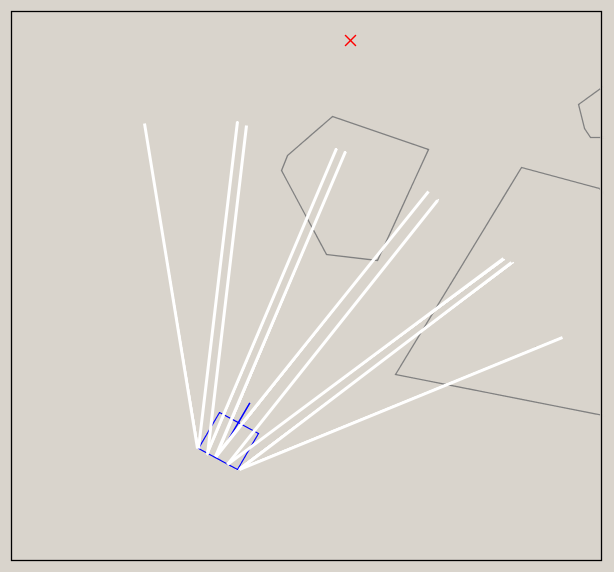
\includegraphics[width=0.4\textwidth]{tank-vis-area}
	\caption{Розташування секторів поля зору в модифікованій задачі}
	\label{fig:tank-vis-area}
\end{figure}

\section{Практичний експеримент}
Оскільки використання попереднього підходу сильно залежить від якості навчальної вибірки (експертних правил), що при найменшому ускладненні сприйняття агентом середовища призводить до значних ускладнень експертних правил, було вирішено відійти від моделі навчання з учителем. Натомість був використаний самоорганізаційний підхід. Основна ідея такого підходу полягає в тому, щоб дати можливість агенту розробити власну систему правил щодо оптимальної поведінки в умовах середовища, завдяки безпосередній взаємодії з середовищем. Взаємодіючи з середовищем, агент отримує певний досвід і, якщо задати певний механізм оцінки агентом власних дій, то в результаті достатньої кількості ``досвіду'', можна надіятися, що агент розробить ефективну стратегію поведінки. Такий підхід отримав назву \emph{навчання з підсиленням (reinforcement learning)}. При використанні навчання з підсиленням відпадає необхідність в складному і трудомісткому процесі розробки системи якісних і репрезентативних експертних правил, хоча, натомість, з'являєть необхідність в виборі механізму оцінки дій агента. Проте, для достатньо складних систем зазвичай значно легше визначити механізм безпосередньої оцінки дій, аніж розробити достатньо повну та якісну систему правил.

Розглянемо застосування такого індуктивного процесу навчання (на відміну від дедуктивного на базі системи правил) до вищезазначеної задачі навігації агента.

\subsection{Середовище}

\begin{figure}
	\centering
    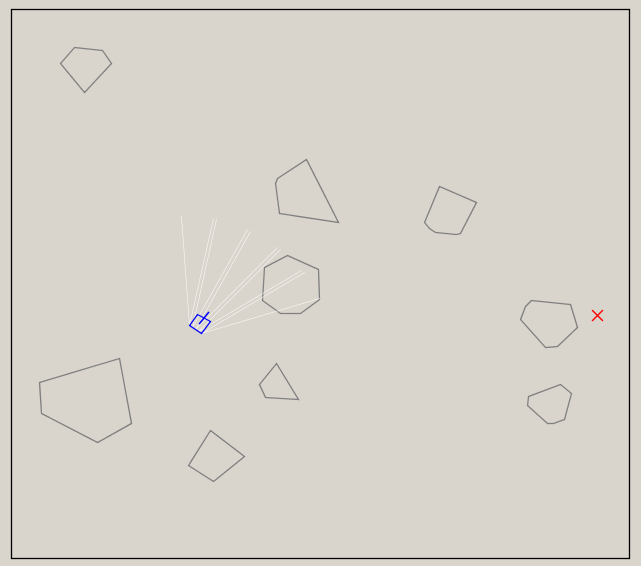
\includegraphics[width=0.7\textwidth]{env_screen.png}
	\caption{Віртуальне середовище}
	\label{fig:environment}
\end{figure}

Для випробування вищезазначеної ідеї було створено віртуальне середовище (див. рис.~\ref{fig:environment}). Робот має п'ять секторів огляду, в межах яких він сприймає точну відстань до найближчої перешкоди. Центральний кут кожного сектору складає 18\textdegree. Таким чином робот сприймає об'єкти в межах поля зору в 90\textdegree. Роботу надається інформація про кут між напрямком його руху та напрямком на ціль, а також відстань до цілі (рис.~\ref{fig:perception}). Таким чином, робот сприймає середовище як багатовимірний неперервний простір.

\begin{figure}
	\centering
    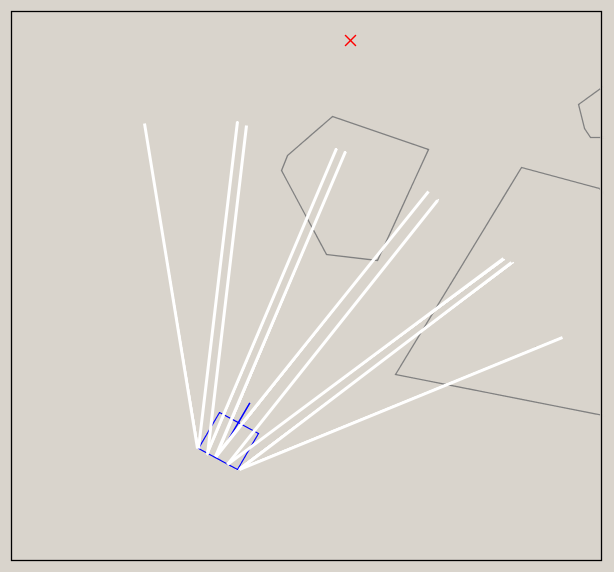
\includegraphics[width=0.7\textwidth]{perception.png}
	\caption{Сприймання роботом середовища}
	\label{fig:perception}
\end{figure}

Середовище становить собою квадратну кімнату, в якій знаходять випадково згенеровані та розташовані перешкоди, що являють собою опуклі многокутники. Уся дія відбувається епізодами. Робот починає на початку кожного епізоду свій рух у випадковій позиції з випадковим початковим напрямом руху і повинен дістатися вказаної точки, яка також генерується випадково, не натикаючись на межі кімнати та на перешкоди.

Робот рухається, вибираючи на кожному кроці дію з дискретної множини допустимих дій, а саме:
\begin{itemize}
	\item рухатись прямо на невелику відстань;
	\item рухатись прямо на невелику відстань, одночасно повернувши наліво на невеликий кут повороту;
	\item рухатись прямо на невелику відстань, одночасно повернувши направо на невеликий кут повороту;
	\item залишитися на місці, повернувши наліво на невеликий кут повороту;
	\item залишитися на місці, повернувши направо на невеликий кут повороту.
\end{itemize}

Робот робить рішення про наступний хід доти, доки не буде виконана одна з наступних умов:
\begin{itemize}
	\item досягнуто цілі;
    \item зіткнення з перешкодою або межею кімнати;
	\item перевищено ліміт кількості кроків;
\end{itemize}

В усіх цих випадках епізод вважається закінченим. Після цього знову генерується випадковий епізод і все повторюється з початку.

\subsection{Деталі реалізації}

В нашій програмній реалізації було використано алгоритм Sarsa для навчання. Параметр дисконтування $\gamma$ було прийнято рівним $0.99$ для того, щоб враховувати якомога краще можливі наслідки прийнятих дій.

За кожен крок агент отримував винагороду, рівну $-0.01$, таким чином ми намагалися домогтися такої послідовності дій, яка б вела до цілі за найменшу кількість кроків. При досягненні мети, отримувалася нагорода, рівна $1.00$. При зіткненні з перешкодою, покарання було найбільшим і становило:
\[
    -1+ \frac{1}{2} e^{-2\frac{d_{crash}}{d_{size}}},
\]
де $d_{crash}$ "--- це відстань від місця зіткнення до перешкоди, $d_{size}$ "--- довжина сторони кімнати.

Таким чином, зіткнення було найнебажанішою подією, але при цьому для того, щоб заохотити робота рухатися в напрямку до цілі, покарання залежало від відстані до цілі. У випадку з перевищенням роботом допустимої кількості дій, покарання було таким же, як і у випадку з зіткненням, проте більшим на $0.3$. Тобто безпечне пересування було пріоритетнішим.

Система винагород була вибрана досить довільно в результаті численних експериментів і з усіх випробуваних варіантів показала себе найефективнішою.

В якості апроксиматора функції була використана нейромережа прямого поширення сигналу, яка на кожній ітерації навчалася за допомогою одного проходу алгоритму зворотнього поширення помилки. Конфігурація нейромережі, використана в нашій програмі: $13-8-1$, при цьому для внутрішніх прошарків використовувалася логістична активаційна функція:
\[
    f(x) = \frac{1}{1 + e^{-x}},
\]
а для вихідного прошарку одинична функція:
\[
    f(x) = x.
\]

Для апроксимації функції $Q(s,a)$ використовувалися 5 окремих нейромереж, кожна з яких відповідала за свою дію. Цей підхід, згідно \cite{Rummery1995}, є дещо ефективнішим, ніж використання однієї нейромережі з кількістю виходів, рівною кількості можливих дій. В такому випадку для ефективної роботи нейромережі достатньо меншої кількості ітерацій навчання, а також меншої кількості нейронів.

Крок навчання $\alpha$ спадав лінійно від $0.3$ до $0.01$, досягаючи мінімуму після одного мільйона навчальних кроків.

На вхід нейромережі подавалися спеціальним чином закодовані 7 відомих параметрів стану: 5 сенсорів відстані для кожного з секторів зору, а також відстань до цілі та кут. Кодування використовувалося те ж саме, що й у \cite{Rummery1995}. Кожен параметр стану кодувався дійсними числами з діапазону $[0,1]$, які обраховувалися за формулою:
\[
    i_n = \frac{1}{1 + e^{w_n(b_n-x)}},
\]
\[
    w_n = \frac{4N}{r},\qquad b_n = \left(\frac{2n-1}{2}\right)\frac{r}{N},
\]
де $N$ "--- кількість входів нейромережі, які відповідають параметру, $r$ "--- це діапазон $[0,r]$, в межах якого вхідні значення будуть найбільш чутливими.

Для сенсорів відстані до перешкоди було вибрано $N = 3$ та $r = 8$. Це дозволило зімітувати обмежену дальність видимості робота, що є значно реалістичніше в реальних застосуваннях, аніж абсолютно точні дані про відстань. Відстань до цілі кодувалася при $N = 5$ та $r = 25$, а відносний кут розбивався на дві частини: $\pi - \varphi$ та $\varphi - \pi$, вводячи поняття ``ціль зліва'' та ``ціль справа'', які кодувалися при $N = 3$ та $r = \pi$.

Ідея такого кодування полягає в тому, щоб при збільшенні важливості значення $x$, збільшувалася кількість ``ввімкнутих'' входів, тобто таких, значення яких близьке до одиниці. Таким чином, чим ближче робот знаходився до перешкоди, тим більше входів активізовувалося. Експеримент показав, що вказане кодування суттєво полегшує задачу навчання і робить його значно ефективнішим та якіснішим.

Усі вагові коефіцієнти нейромережі були початково ініціалізовані нулями, що завдяки одиничній функції у вихідному прошарку, початково давало значення нуль для будь-якого входу. Це є досить важливим моментом. В літературі (\cite{SuttonBarto2002}) рекомендують при можливості використовувати таке початкове наближення функції корисності $Q(s,a)$, яке б було оптимістичним, по відношенню до реальної функції вартості. В такому випадку агент, вибравши певну дію і отримавши винагороду, яка є нижчою, ніж початкове оптимістичне наближення, наступного разу в тій же ситуації буде схилятися до вибору іншої дії, таким чином пробуючи кожного разу іншу дію. Все це забезпечить швидше та більш точне наближення реальної ціннісної функції.

В нашому випадку, робот спочатку діє дуже неефективно. Оскільки ймовірність добратися до цілі, минаючи перешкоди, в умовах випадково згенерованого середовища дуже невелика, то початково постійно буде отримуватися негативне значення винагороди. Тому нульова ініціалізація нейромережі становить собою оптимістичні сподівання, і, відповідно, є корисною евристикою.

Щодо конкретних параметрів середовища та робота, то вони наступні. Робот становить собою квадрат розміром $1 \times 1$, середовище "--- також квадрат розмірністю $40 \times 40$. Сприймання перешкод відбувалося в межах п'яти секторів, кожен з кутом 18\textdegree, тобто сумарно поле зору становило 90\textdegree. Вважалося, що робот досягнув цілі, якщо він знаходився на відстані меншій $1$ від цілі. Зіткнення зараховувалося при відстані меншій $0.01$. На кожному кроці робот міг рухатися вперед на відстань $0.9$.

Розташування перешкод в кімнаті генерувалося автоматично, при цьому випадковим чином вибиралася кількість перешкод з діапазону $[4,10]$, для кожної перешкоди випадково генерувалася позиція її центру та радіус з діапазону $[1.5, 4.0]$.

\subsection{Результати}

Практичні експерименти показали, що агенту достатньо $1.2$ мільйонів кроків навчання для того, щоб вивчити власну стратегію, після чого вона практично не змінюється. Ефективність контролера оцінювалася у відсотках успішних добирань до цілі за останні $5000$ епізодів, щоб знівелювати вплив фактично випадкових неадекватних дій на початку навчання.

Початково значення $\varepsilon$ у $\varepsilon$-жадібній стратегії було фіксованим на позначці $0,1$, що становило собою розумний компроміс між випадковістю поведінки та можливістю дослідження ``нерозвіданих'' стратегій. При цьому вершини секторів, які відповідали за зір робота, починалися у центральній точці робота. Таке поєднання налаштувань дозволяло агенту досягати успішності в $60\%-65\%$ випадків. При цьому робот поводив себе цілком адекватно, стараючись оминути перешкоди, проте часто зачіпаючи боковою стороною краї перешкоди. Це зумовлено обмеженістю поля зору (див.рис.~\ref{bad_perception}), оскільки сектори захоплювали лише ту частину простору, яка знаходилася безпосередньо перед роботом, ніяк не даючи знати про перешкоди, що знаходяться в безпосередній близькості збоку.

\begin{figure}
	\centering
    \subfloat[Початковий варіант]{\label{bad_perception}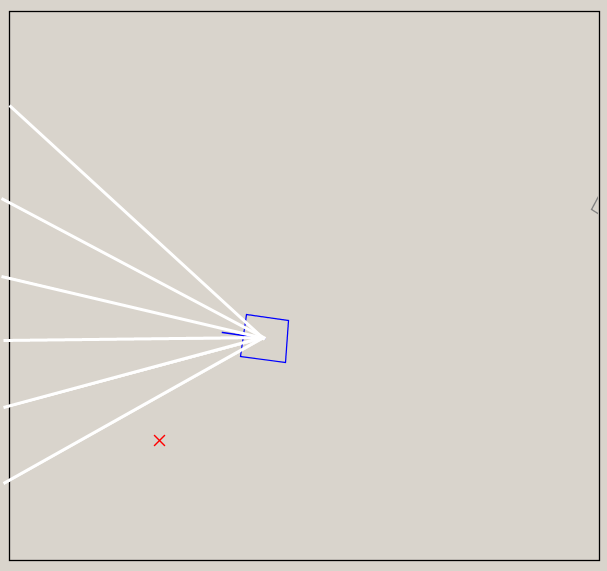
\includegraphics[width=0.45\textwidth]{bad_perception} }
	\;
    \subfloat[Більш ефективний варіант]{\label{good_perception}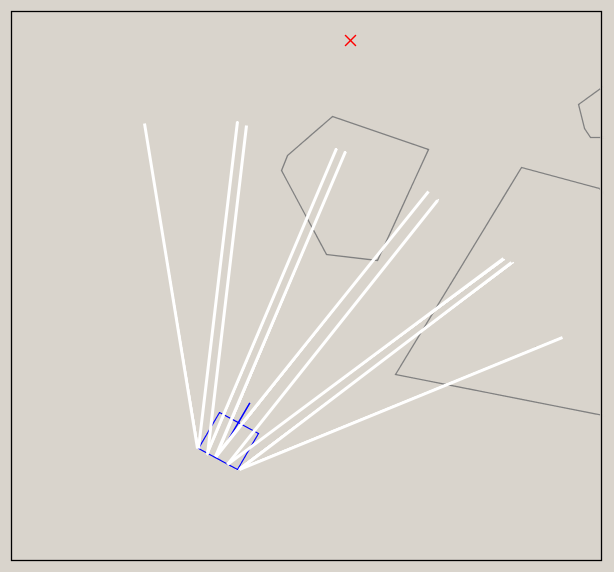
\includegraphics[width=0.45\textwidth]{perception}}
	\caption{Різні форми області сприймання перешкод}
	\label{bad_and_good_perception}
\end{figure}


Для того, щоб дати більше інформації про оточуючі перешкоди, поле зору робота було дещо видозмінене (див. рис.~\ref{good_perception}). Вершини секторів були зміщені в задню частину і рівномірно розподілені по всій задній стороні. Таким чином, у робота тепер були два сектори, які надавали йому інформацію про дуже близькі перешкоди, що знаходилися ліворуч та праворуч від нього. Ці вдосконалення дозволили підвищити успішність агента до позначки $80\%-82\%$ в більшості тестових запусків. Аналіз нової стратегії показав, що поведінка робота дійсно стала значно безпечнішою та ефективнішою. Але при цьому часто можна було спостерігати як робот оминає перешкоду, об'їжджаючи її ``впритул'', і час від часу здійснює випадкові повороти в сторону перешкоди. Це було зумовлено тим, що значення ймовірності вибору випадкової дії $\varepsilon$ було вибрано досить великим "--- $0.1$. Тобто в середньому в одному випадку з десяти агент здійснював випадковий вибір дії, що призводило до зіткнень при близькості до перешкоди.

Зменшення $\varepsilon$ до $0.01$ призвело до значного погіршення навчального процесу, оскільки алгоритму Sarsa не надавалося достатньої можливості досліджувати нові стратегії, натомість поведінка агента збігалася до локального мінімуму, який був далекий від оптимального.

В результаті цих спостережень ми вирішили використати змінний показник $\varepsilon$, який лінійно спадав від $0.2$ до $0.01$ протягом 1 мільйону кроків навчання, після чого фіксувався на мінімальній позначці. Таке вдосконалення повинно було б допомогти агенту на початку дослідження більш повно досліджувати можливі нерозвідані дії, при цьому зменшуючи ймовірність вибору неоптимальних дій тоді, коли в результаті багатьох ітерацій, вивчена функція цінності давала хороше уявлення про оптимальні дії і необхідність в дослідженні випадкових дій зникала.

Експеримент показав, що таке вдосконалення дійсно дає краще результати. З усіма вищезазначеними вдосконаленнями в 8 випадках із 10 успішність агента становила $87\%-92\%$ успішних епізодів.

На рис.~\ref{fig:bad-moves-samples} показано траекторії робота без будь-якого навчання.
\begin{figure}
  \centering
  \subfloat{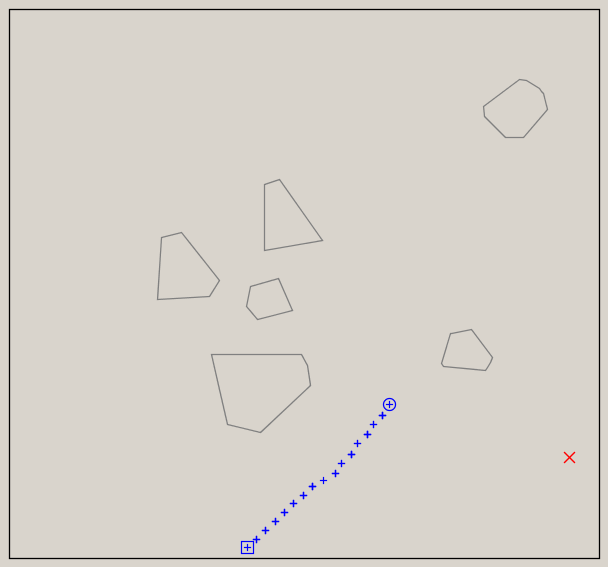
\includegraphics[width=0.47\textwidth]{bad1}}\,
  \subfloat{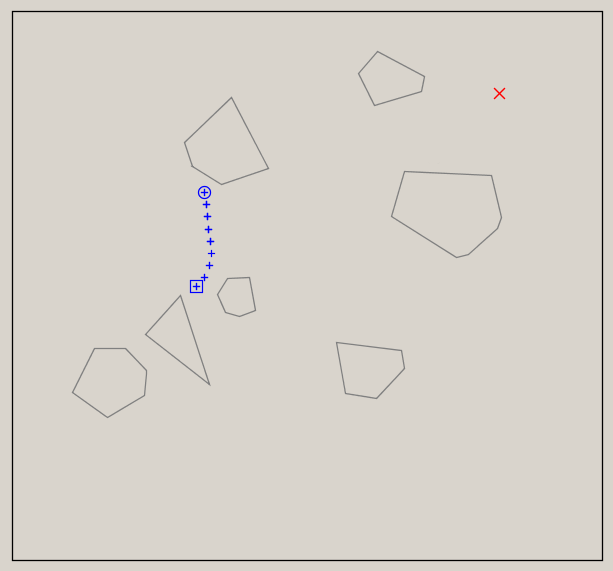
\includegraphics[width=0.47\textwidth]{bad2}} \\
  \subfloat{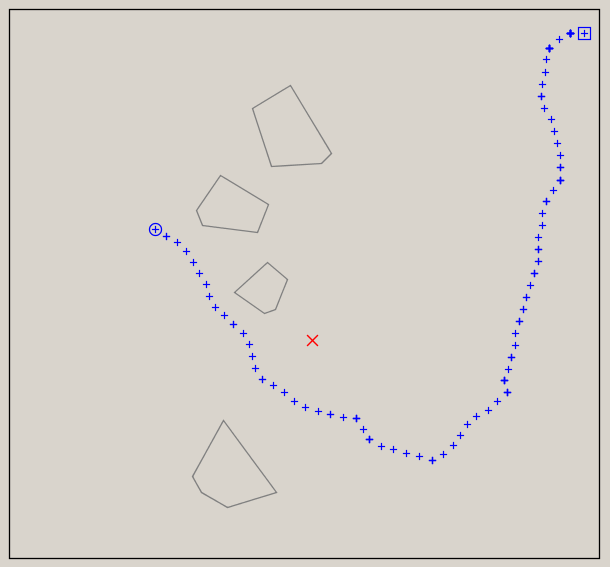
\includegraphics[width=0.47\textwidth]{bad3}}\,
  \subfloat{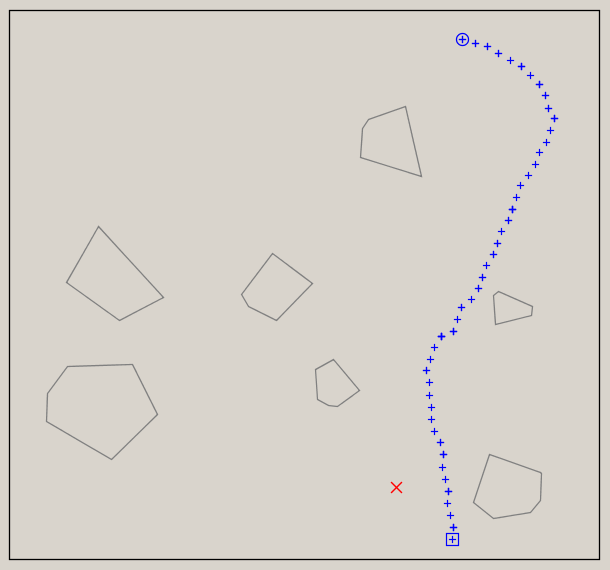
\includegraphics[width=0.47\textwidth]{bad4}}
  \caption{Приклади початкових траекторій без навчання}
  \label{fig:bad-moves-samples}
\end{figure}

На рис.~\ref{fig:samples-samples} показано приклади траекторій робота на проміжних стадіях навчання.

\begin{figure}
  \centering
  \subfloat{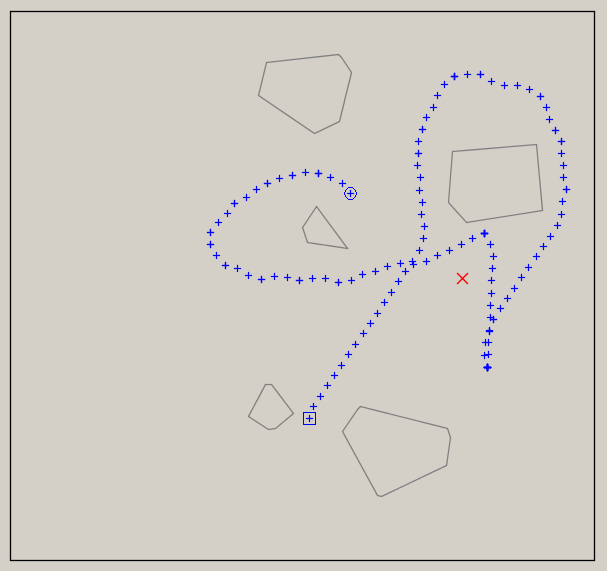
\includegraphics[width=0.47\textwidth]{in_the_middle_of_learning}}\,
  \subfloat{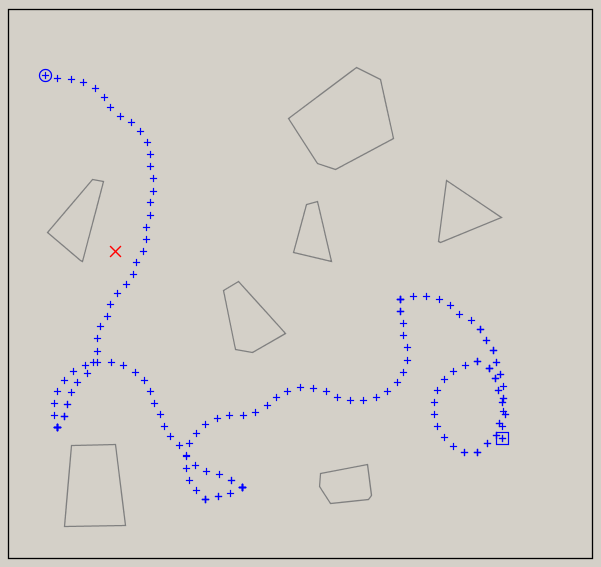
\includegraphics[width=0.47\textwidth]{in_the_middle_of_learning2}} \\
  \subfloat{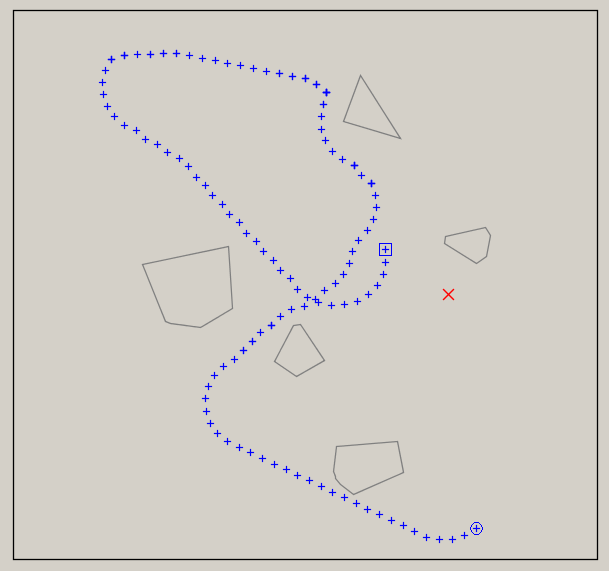
\includegraphics[width=0.47\textwidth]{sample}}\,
  \subfloat{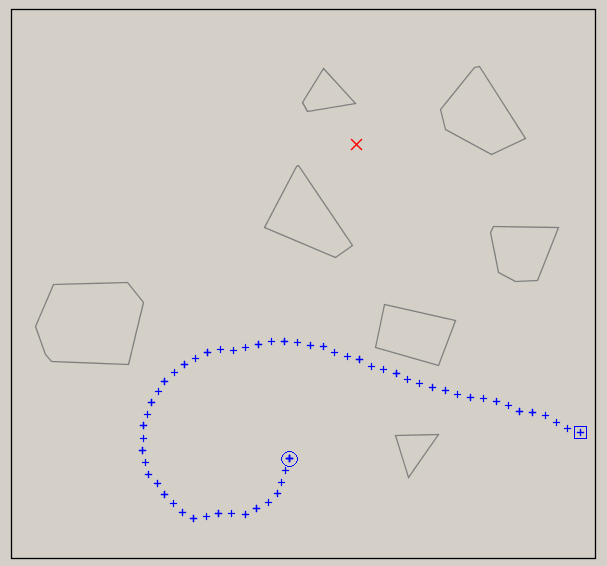
\includegraphics[width=0.47\textwidth]{env2_not_learned}}
  \caption{Приклади траекторій на проміжних стадіях навчання}
  \label{fig:samples-samples}
\end{figure}

На рис.~\ref{fig:learning-samples} наведено приклади траекторій в умовах однієї і тієї ж кімнати після різної кількості навчальних кроків.
\begin{figure}
  \centering
  \subfloat[Без навчання]{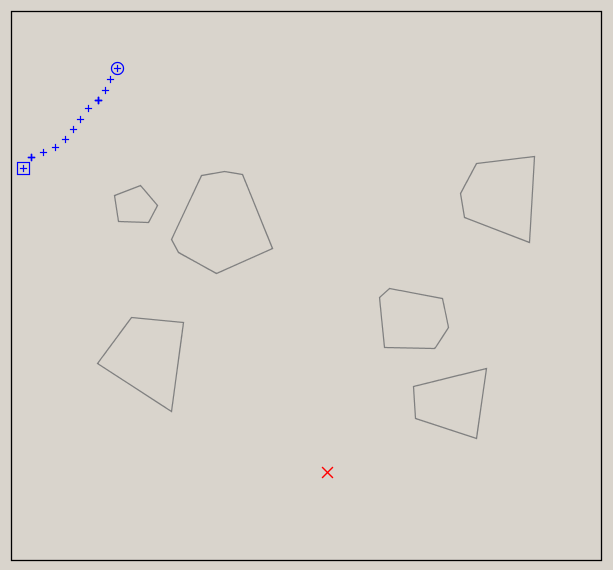
\includegraphics[width=0.47\textwidth]{learn1}}\,
  \subfloat[Після $100$ тис. ітерацій]{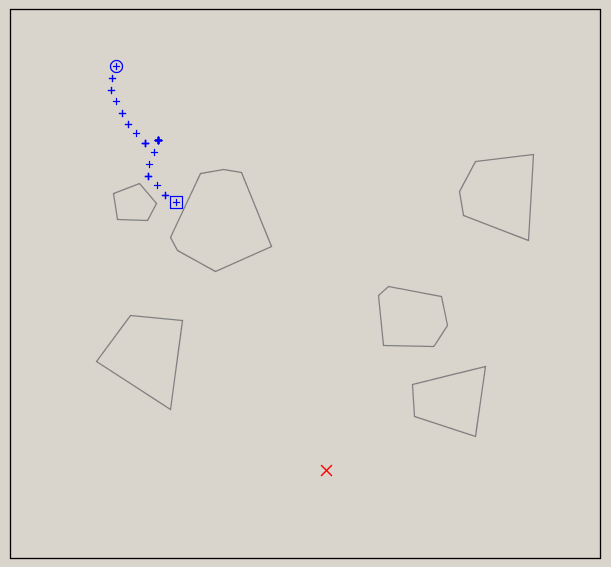
\includegraphics[width=0.47\textwidth]{learn2}} \\
  \subfloat[Після $500$ тис. ітерацій]{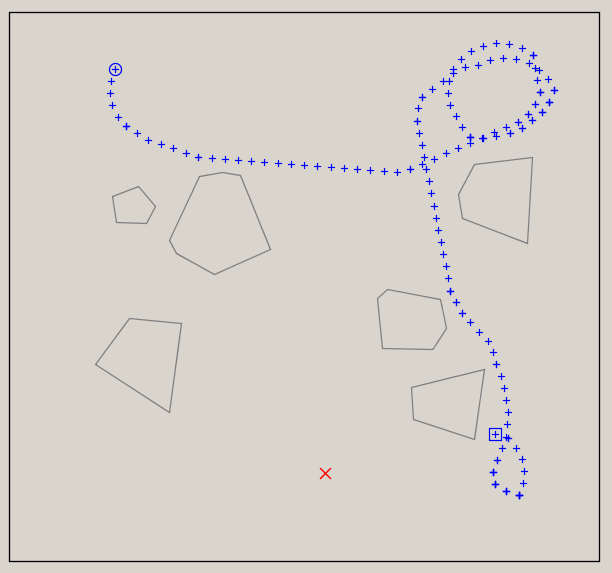
\includegraphics[width=0.47\textwidth]{learn3}}\,
  \subfloat[Після $1.2$ млн. ітерацій]{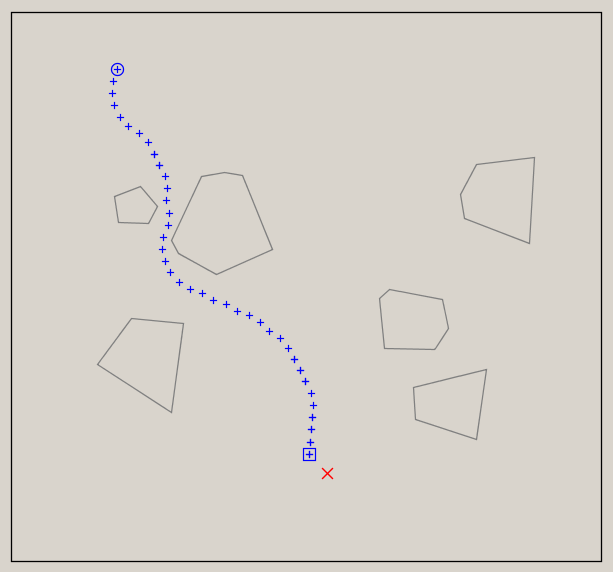
\includegraphics[width=0.47\textwidth]{learn4}}
  \caption{Приклади траекторій в умовах одного і того ж середовища}
  \label{fig:learning-samples}
\end{figure}

На рис.~\ref{fig:success-samples} показано приклади траекторій робота після навчання.

\begin{figure}
  \centering
  \subfloat{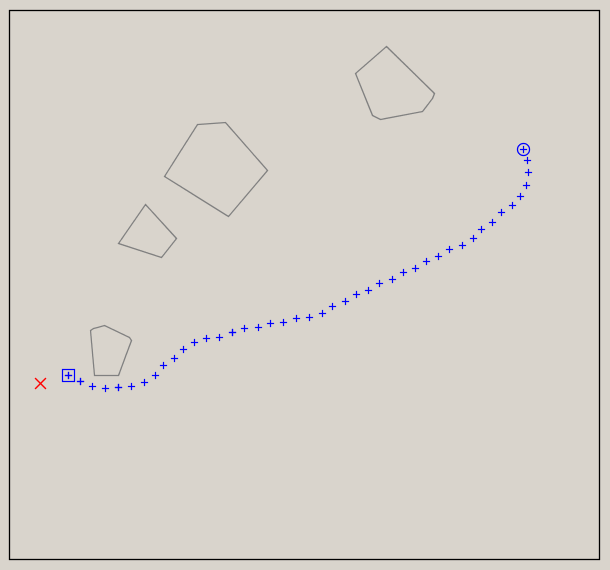
\includegraphics[width=0.47\textwidth]{good1}}\,
  \subfloat{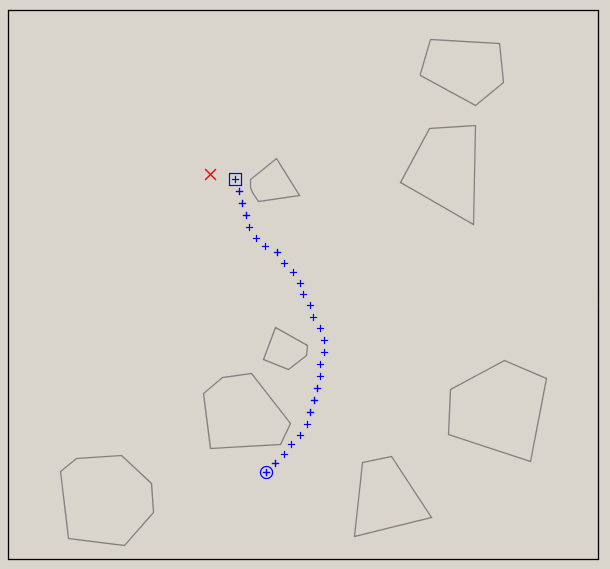
\includegraphics[width=0.47\textwidth]{good2}} \\
  \subfloat{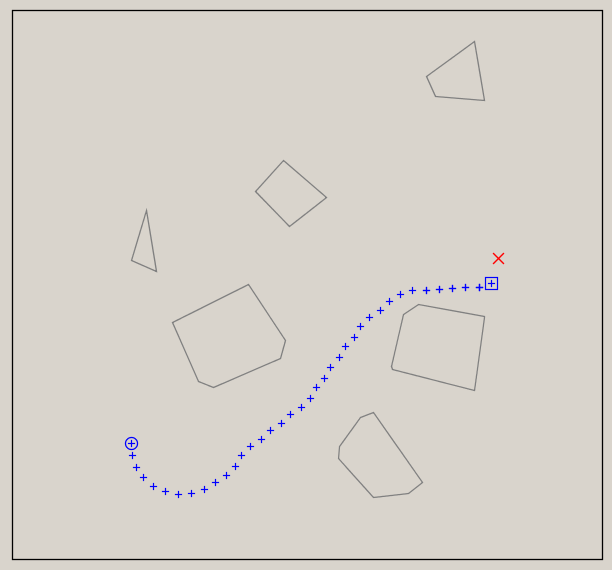
\includegraphics[width=0.47\textwidth]{good3}}\,
  \subfloat{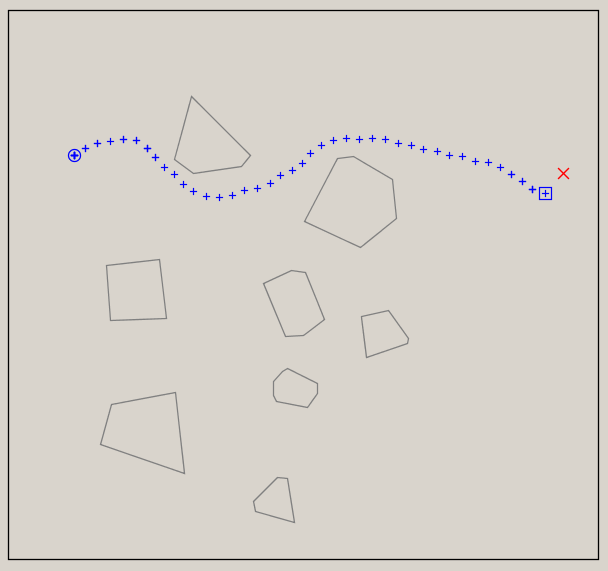
\includegraphics[width=0.47\textwidth]{good4}}
  \caption{Приклади траекторій навченого робота (після 1.2 мільйона навчальних кроків)}
  \label{fig:success-samples}
\end{figure}

На всіх цих ілюстраціях символом + позначено рух робота, + в квадраті "--- фінальна позиція робота, + в крузі "--- початкова позиція робота, x "--- ціль.

\section{Висновки}

Використовуючи парадигму навчання з підсиленням, було створено адаптивний контролер навігації робота, який базуючись на обмеженій інформації про навколишній світ, забезпечує добирання робота до цілі, оминаючи зіткнення з перешкодами. Як показали практичні експерименти, розроблений контролер є ефективним і забезпечує успішне добирання до цілі в абсолютній більшості випадків (в середньому $87\%-92\%$).

Якщо порівнювати використаний підхід, з попереднім підходом на базі системи експертних правил, використаним нами раніше, можна відзначити, що навчання з підсиленням забезпечує значно більшу гнучкість, даючи можливість змінювати структуру стану системи, без жодних інших ускладнень. У випадку з системою експертних правил, така зміна одразу приводить до труднощів, оскілько потрібно розробляти абсолютно нову систему правил, що є надзвичайно трудомістким та складним процесом. На жаль, досить важко в кількісному відношенні порівняти два зазначених підходи, оскільки, по-перше, цілі в цих двох задачах були дещо різні: просто оминання перешкод в випадку з системою правил та добирання до цілі з оминанням перешкод у випадку з навчанням з підсиленням. По-друге, фізика моделей автомобіля та робота суттєво відрізняється, що унеможливлює об'єктивне порівняння. Проте, суб'єктивно, поведінка самостійно навченого робота виглядає значно раціональнішою, природнішою та більш адекватною, порівняно з поведінкою автомобіля у схожих ситуаціях (наприклад, при під'їзді до близько розташованої перешкоди).

Cлід зазначити, що в обидвох підходах є як позитивні, так і негативні сторони. Для підходу на базі експертних правил характерним є швидкий процес навчання, проте сама розробка правил досить громіздка. Для навчання з підсиленням навпаки: немає затрат часу та сил на розробку системи правил, оскільки мобільний агент сам розробляє свої внутрішні правила, проте процес навчання триває досить довго. Для прикладу, здійснення 2 мільйонів навчальних кроків на середньостатистичному комп'ютері триває більше години часу. Неоднозначним для навчання з підсиленням є його залежність від евристичних параметрів: зміна параметру $\varepsilon$ у $\varepsilon$-жадібній стратегії вибору дій з константного значення $0.1$ на лінійно-спадну послідовність від $0.2$ до $0.01$ призвело до покращення результатів на $5\%-10\%$.

Можливо, саме така залежність навчання з підсиленням від евристичних параметрів є поясненням того, що розроблена нами система контролю за своїми показниками уступає від аналогічної системи, розробленої G.A.Rummery(\cite{Rummery1995}), для якої характерними були показники рівня успішності робота в межах $96\%-99\%$. Очевидно, більш якісним підбором різноманітних евристичних параметрів навчання, можна було б досягти ефективнішої роботи контролера.

Тим не менше, зручність та легкість внесення будь-яких змін у структуру середовища, його стану чи фізики моделі без зміни навчального процесу, а також хороші показники ефективності роботи навченого контролера "--- безсумнівні переваги навчання з підсиленням. У випадку з проблемою навігації, незначна зміна сприймання роботом навколишнього середовища таким чином, щоб поле зору захоплювало незначну територію зліва та справа від нього, без будь-яких інших вдосконалень дає покращення результатів на $15\%-17\%$. 

Особливої уваги заслуговує використання штучної нейромережі у якості апроксиматора функції. Хороші властивості апроксимації та узагальнення нейромережі "--- основна складова успішного застосування навчання з підсиленням для складних проблем з неперервним простором станів, як у випадку з навігацією робота. У нашому випадку нейромережа показала себе чудовим інструментом, який доповнює парадигму навчання з підсиленням. Цікавим є те, що, незважаючи на те, що в літературі досі не було дано будь-яких теоретичних доведень збіжності алгоритмів навчання з підсиленням при умові використання нелінійних апроксиматорів функцій, вкотре було показано практичну застосовність поєднання штучних нейромереж та алгоритму навчання з підсилення (зокрема, Sarsa) для складних задач контролю. 

Проте, нейромережа вносить додатковий рівень складності у розроблені алгоритми, вимагаючи обережного та точного підбору параметрів навчання самої нейромережі, а також вибору оптимальної структури, кількості нейронів та їх активаційні функції. 

Серед майбутніх напрямків роботи можна зазначити зміну завдання агента з добирання до вказаної цілі на завдання оптимального покриття обмеженого простору (кімнати) з оминаннями перешкод. Такий агент може бути корисним для використання у побутовій робототехніці, наприклад, для створення робота-порохотяга. В цьому ж руслі слід відзначити можливість використання різноманітних промислових сенсорів, наприклад, ехолокаторів, датчиків руху тощо. Успішне поєднання цих пристроїв з індуктивним навчанням приблизить нас до застосування розроблених методів у реальних пристроях, а не у віртуальних програмних середовищах.

Ще одним напрямком досліджень слід відзначити продовження дослідження в царині навчання без учителя. Одним з таких напрямків є ієрархічне навчання з підсиленням, яке зосереджується на тому, щоб залежно від стану агента та системи, перемикатися на виконання найбільш актуального та критичного завдання. Наприклад, у випадку з автономним роботом-порохотягом, якщо стан акумулятора буде свідчити про низький рівень заряду, то найбільш актуальним завданням для робота стане пошук найближчої док-станції, а не покриття кімнати.

Загалом, індуктивні методи навчання є дуже перспективним напрямком роботи, оскільки дають можливість створювати достатньо ефективні контролери для задач, з якими дедуктивні методи не справляються в силу надзвичайної складності поставленого завдання.

\addcontentsline{toc}{section}{Література}
\begin{thebibliography}{99}
\bibitem{Rummery1995}{Rummery, G. A. 1995. Problem Solving with Reinforcement Learning. Ph.D. thesis. Cambridge University Engineering Department.}
\bibitem{SuttonBarto2002}{Sutton, R. S., Barto, A. G. 2002. Reinforcement Learning: An Introduction. A Bradford Book, The MIT Press, Cambridge, Massachusetts, London, England.}
\bibitem{Coulom2002}{Coulom, R. 2002. Reinforcement Learning Using Neural Networks, with Applications to Motor Control. Ph.D. thesis. Institut National Polytechnique de Grenoble.}
\bibitem{Kaelbling1996}{Kaelbling L., Littman M., Moore A. 1996. Reinforcement Learning: A Survey. Journal of Artificial Intelligence Research 4, 1996, 237-285}
\bibitem{Tesauro1995}{Tesauro G. 1995. Temporal Difference Learning and TD-Gammon. Communications of the ACM, March 1995 / Vol. 38, No. 3}
\bibitem{Kun03}{Phіlіppe Kunzle. Vehіcle Control wіth Neural Networks "--- http://www.gamedev.net/reference/artіcles/artіcle1988.asp}
\bibitem{WikiMDP}{Wikipedia. Markov Decision Process "--- http://en.wikipedia.org/wiki/Markov\_decision\_process}
\end{thebibliography}

\end{document}
